\documentclass[10pt,a4paper]{article}
\usepackage[utf8]{inputenc}
\usepackage{amsmath}
\usepackage{amsfonts}
\usepackage{amssymb}
\usepackage{graphicx}
\usepackage{subfigure}
\usepackage{amsmath}
\usepackage{mathrsfs}
\DeclareRobustCommand{\orderof}{\ensuremath{\mathcal{O}}}
\bibliographystyle{prsty}
\usepackage[top=1in, bottom=1in, left=1in, right=1in]{geometry}

\begin{document}
\section{Introduction}


\textbf{hop} is a key task of PiLab. It generates all tight-binding parameters of the system. This task will first assign the orbitals\footnote{Here we use the term ``orbital'' to represent $s$, $p$, $d$, $f$ and ``suborbital'' to represent a particular component of them. For example, $p_{x}$, $p_{y}$ and $p_{z}$ are suborbitals of the $p$ orbital}    of each sublattice. Then \textbf{hop} will automatically generates the hopping integrals using Slaster-Koster methods. If spin-orbit coupling is assumed, \textbf{hop} will also generate onsite spin-orbit coupling matrix. When all the interaction matrices are generated, \textbf{hop} can also transform their basis set. By default, it is in cubic harmonics. If needed, one can transform them to spherical harmonics, relativistic spherical harmonics and relativistic cubic harmonics\footnote{For the definition of each basis in PiLab, one should reference the ``basis\_set.pdf" file for details.}. Using correct basis set will help users to input the onsite energy based on their crystal field splitting easily. 

In most tight-binding calculation, not all the suborbitals are needed. For example, people usually consider $p_{z}$ only rather than the full $p$-orbital when studying graphene systems. In \textbf{hop}, there is also a keyword for users to select the suborbitals they want. 

\section{Dictionary}

\subsection{Input}
\textit{\textbf{hop.SiteOrb}} This parameter assigns the orbital on each sublattice. Each orbital is specified by two values [sublattice index, orbital quantum number]. Sublattice index is defined by the order of the sublattice in lat.Sublatt of the \textbf{lat} task. orbital quantum number are 0 for $s$, 1 for $p$, 2 for $d$ and 3 for $f$ orbitals.For example, [1,1;1,1;2,2] means there are two $p$ orbitals on sublattice 1 and one $d$ orbital on sublattice 2. \\ \\ 
\textit{\textbf{hop.Order}} This parameter sets the order of the hopping integrals. If hop.Order=1, \textbf{hop} will only calculates the hopping between first nearest sites. Similar, if hop.Order=2, it will calculate the hopping integrals between first and second nearest site. Obviously, this parameter has to be smaller or equal to lat.Order, i.e. \textbf{lat.Order} $\leq$ \textbf{hop.Order}, due to the lack of higher order lattice information. The benefits of using this parameter is for user to quickly compare the difference between 1st and 2nd hopping effects. Even though 2nd order hopping in input, \textbf{hop} will still set all 2nd order hopping integrals zero if this parameter is set to 1.\\ \\
\textit{\textbf{hop.SKint}} This parameter sets the hopping integrals. When two orbitals overlap to  each other, their hopping integrals can be specified by just a few parameters, i.e the strength of the bonds with different symmetry. For example, when two $p$-orbitals couple to each other, $\sigma$-bond and $\pi$-bond will be formed. If these two bond strengths are given, the hopping integrals between arbitrary suborbitals as a function of bonding angles can be evaluated using Slaster-Koster formulation\footnote{see, Phys. Rev. 94 1498, J. Phys. C. 13 583 for details. Also see Slaster\_Koster.pdf for the exact formulas used in PiLab.}. There are four Slaster-Koster integrals or, in other words, four different bonds which are called $\sigma$, $\pi$, $\delta$ and $\phi$ bond respectively. However, not all of them are needed to specify the coupling between two orbitals. Consider that each bond has the same symmetry as the $s (\sigma)$, $p (\pi)$, $d (\delta)$ and $f (\phi)$ orbital respectively. When two orbital couple to each other, only the minimal symmetry will be held. For example, $s-s$ has $\sigma$ bond only, $p-p$ has both $\sigma$ and $\pi$. However, $s-p$ will have $\sigma$ only. Similarly, $d-d$ has $\sigma$, $\pi$, $\delta$ bonds, but $p-d$ has only $\sigma$, $\pi$. In this parameter, we will need 7 input values to specify the bond strength between two orbitals [orbital label 1, orbital label 2, hopping order, $\sigma$, $\pi$, $\delta$, $\phi$]. Orbital labels are the orbitals defined in hop.SiteOrb. 1 corresponds to first orbital defined in hop.SiteOrb and so on. Hopping order is the order of the two orbitals. $\sigma$, $\pi$, $\delta$ and $\phi$ are the bond strength. Even though not all bonds exist, you should still give the non-existed bonds values, e.g. zero. This is just to make the size of the input parameters consistent. No matter what are the values for the non-existed bonds, PiLab won't use them. For example, [1,2,1,2,1,0,0] means the orbital 1 and orbital 2 defined in hop.SiteOrb have $\sigma$ bonding strength = 2 and $\pi$-bond strength = 1 if they are on first nearest sites. Of course, it is possible that two orbitals overlapped with second nearest sites. If so, set hopping order = 2. If you need to input more hopping integrals, separates each set via semicolon ";". An important restriction of this parameter is that \textbf{orbital label 1 must smaller or equal to orbital label 2} and PiLab will automatically generate the swapped case. For example, [2,1,1,2,1,0,0] is not allowed because once [1,2,1,2,1,0,0] is input, PiLab will generate [2,1,1,2,1,0,0] automatically and the user shoud not input it again.  \\ \\
\textit{\textbf{hop.LS}} This parameter sets the strength of spin-orbit coupling. The Hamiltonian reads $H_{SO}=\alpha \textbf{L} \cdot \textbf{S}$. This parameter gives $\alpha$.\\ \\
\textit{\textbf{hop.Filiter}} This parameters sets the value to filter out small hopping integrals. By default, this value is set to be $10^{-3}$. Therefore, any hopping integrals whose absolute values are smaller than it will be set to zero. It helps user to make the hopping matrix more readable. \\ \\  
\textit{\textbf{hop.Basis}} This parameter sets the orbital basis of the Hamiltonian. 'c' for cubic harmonics, 's' for spherical harmonics, 'rs' for relativistic spherical harmonics and 'rc' for relativistic cubic harmonics. Using appropriate basis will help you input the onsite energy based on crystal field splitting easier. \\ \\
\textit{\textbf{hop.SelState}} This parameter select the suborbitals. If one wants to select just a few suborbitals from the calculations, one should leave it empty and run \textbf{hop} task first. Once it is done, the output variable \textbf{hop.state\_info\_text} will show you all the suborbitals and their state labels. Check what suborbitals you want to keep and input their state labels in this parameter and the onsite energy of these states in \textbf{hop.OnsiteE}. Then run it again. PiLab will automatically kick out all non-selected suborbitals and regenerates the \textbf{hop} file again. \\ \\
\textit{\textbf{hop.OnsiteE}} This parameter sets the onsite energy of each suborbital. By default, PiLab will set all onsite energy as zero. Once hop.SelState is set, hop.OnsiteE will give the onsite energies of each selected state. For example, if we've picked state [1,3,5], then hop.OnsiteE=[-1,-2,-3] means their onsite energies are -1, -2, -3 respectively. If you leave it empty, then all the onsite energies of the selected states are assumed to be zero. Note that, even if you don't want kick out any suborbitals and just want to input onsite energies, you will still need to select all states. hop.OnsiteE will not be functional unless hop.SelState is set. \textbf{Here "..." is the keyword for line change in Scilab}. When this keyword occurs, Scilab will consider the current line and its next line as the same line. It is useful to deal with long input case.

\subsection{Output}
\textit{\textbf{hop.state\_info\_text}} This variable shows all the quantum mechanical states (suborbitals) in the system. There are 5 strings in each row column [state\_label, site, orbital identifier, orbital quantum number, text of suborbital]. State\_label labels the number of each state. This number is also used to expand all the Hamiltonian matrices. In all later tasks, these numbers will also be used as the label of states. Site is the sublattice which this state belongs to. orbital identifiers are the order of each orbital input in hop.SiteOrb. So, two orbitals with the same orbital quantum numbers on the same site will still have different identifiers to distinguish them. Orbital quantum numbers are the same with the definition in hop.SiteOrb. Text of suborbital is a text description of the state. It contains three information: the suborbital number, the orbital quantum number in text form ($s$, $p$, $d$ $f$) and the suborbital in text form. suborbital number is the number that PiLab used in the code to represent a suborbital. Since $s$, $p$, $d$ $f$ have 32 suborbitals in total (including spin), PiLab uses a number to represent each suborbital. This information is not that important if you are not going to develop PiLab project. Therefore, [1 \# 1 \# 1 \# 2 \# 9 D xy,d \#] means state 1 is located in sublattice 1. Its orbital identifier is 1 and it is the spin-down $xy$ component of a $d$ orbital.\footnote{For the definition and notation of each suborbital, see suborbital.pdf for details}  \\ \\
\textit{\textbf{hop.state\_info}} This variable is the numerical format of hop.state\_info. It is what PiLab really uses to deal with suborbitals in the code. For most users you can just ignored this part. \\ \\
\textit{\textbf{hop.LS\_mat}} This variable is the LS coupling matrix. Since $H_{SO}$ is a harmitian matrix, PiLab will output only the upper triangle part by sparse format. \\ \\
\textit{\textbf{hop.onsite\_E}} This variable is the onsite energy matrix. Since $H_{onsite}$ is a diagonal matrix, PiLab will output it by sparse format. \\ \\
\textit{\textbf{hop.hop\_size}} This variable is the size of variable hop.hop\_mat. It is just to help PiLab to preset the memory size if hop.hop\_mat is loaded by other tasks. For most users, this variable can be ignored. \\ \\
\textit{\textbf{hop.hop\_mat(n)(:,:,m)}} This variable is the the hopping integrals between two orbitals. n represents the sublattice label and m represents the m-th neighbor site shown in lat.surr\_site(n). Therefore, hop.hop\_mat(1)(:,:,2) is the hopping between sublattice 1 and its 2nd neighbor, i.e the site defined by the 3rd row vector (1st row vector is the sublattice itself so it is not considered as a neighbor) of the of the variable lat.surr\_site(1). Obviously, their hopping matrix is not hermitian because it just records the hopping from sublattice n to its m-th neighbor site. However if you combine the hopping matrix from m-th neighbor site to sublattice n, it will be hermitian. Since the hopping matrix is zero for most matrix elements, PiLab shows it in sparse format. Note that, this is the sparse matrix of the full hopping matrix rather than the upper triangle part only. \\ \\


\begin{figure}[tbp]
\centering
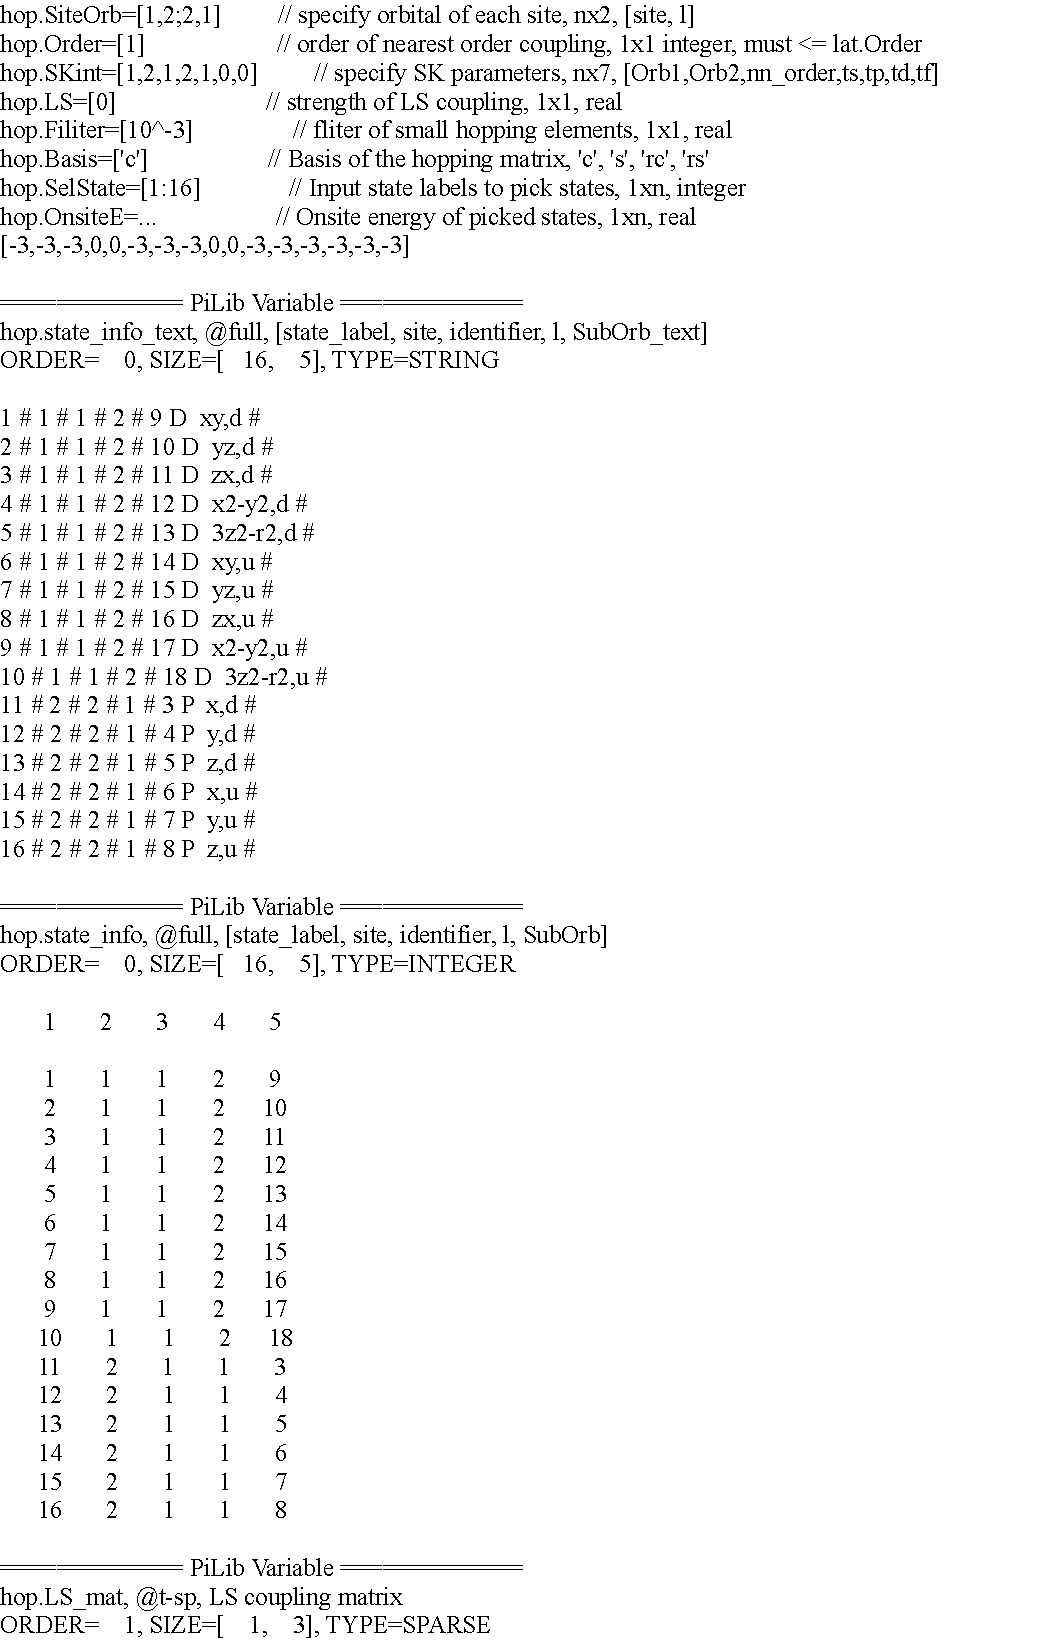
\includegraphics[width=0.9\columnwidth]{NiO_hop_p1.pdf}
\caption{page 1 of NiO\_hop.plb}
\end{figure}

\begin{figure}[tbp]
\centering
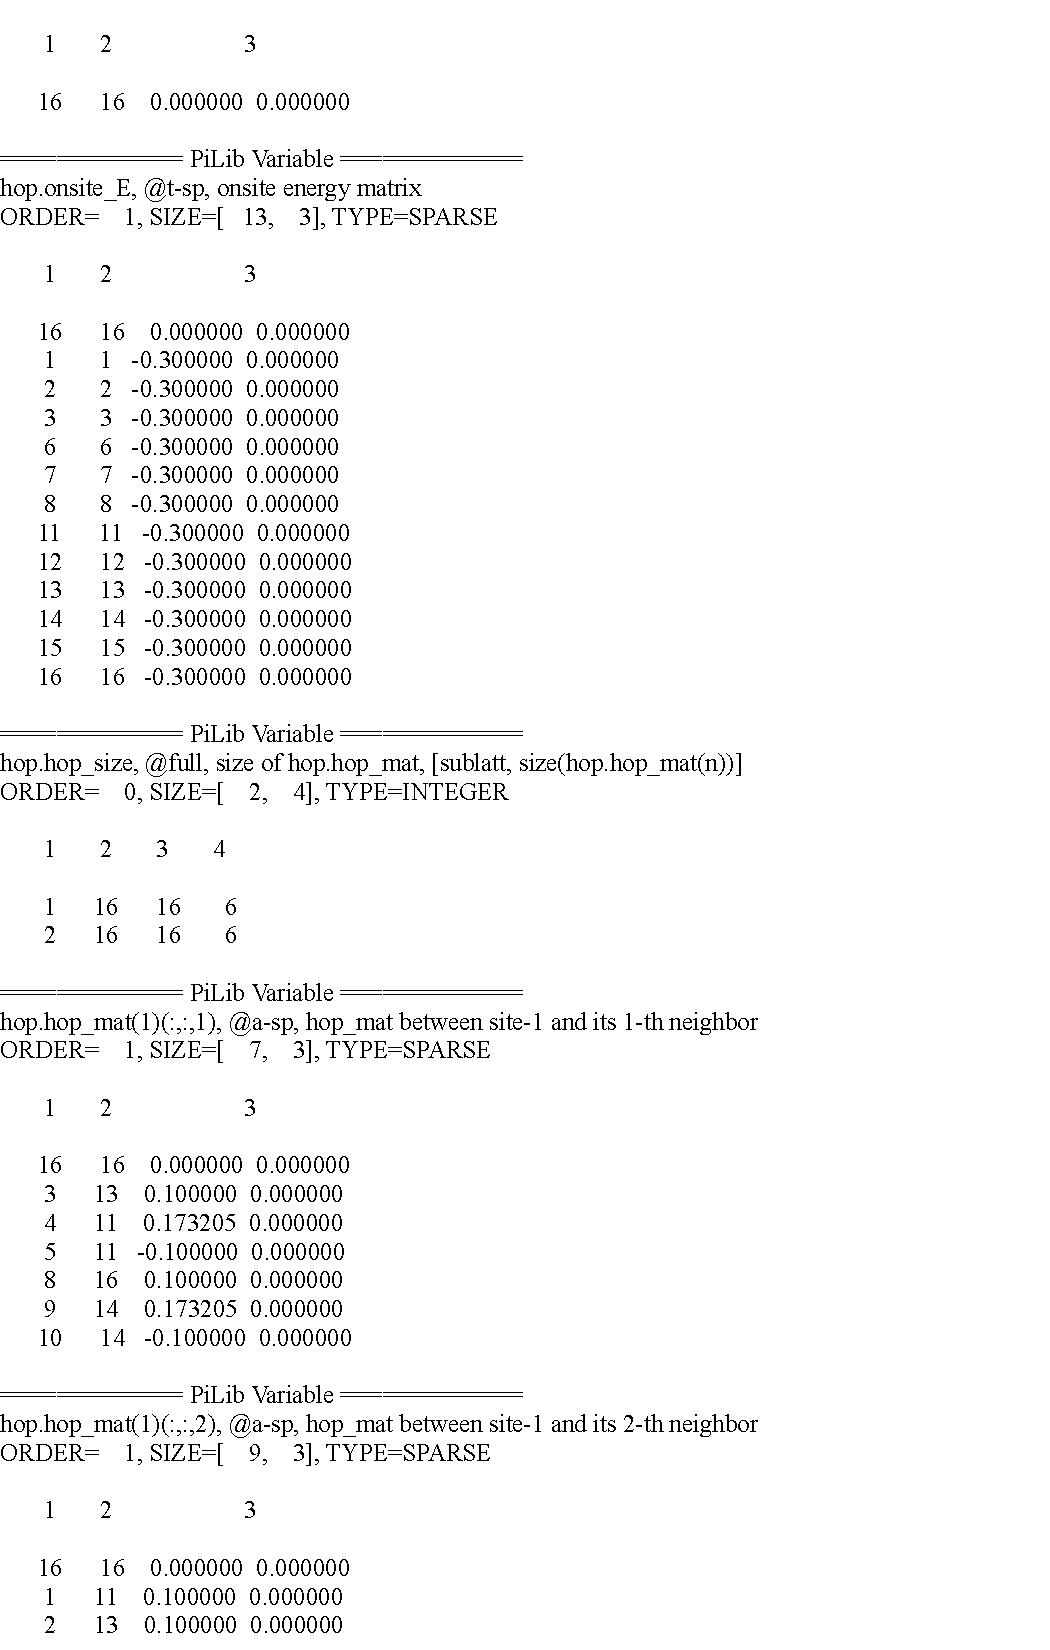
\includegraphics[width=0.9\columnwidth]{NiO_hop_p2.pdf}
\caption{page 2 of NiO\_hop.plb}
\end{figure}

\begin{figure}[tbp]
\centering
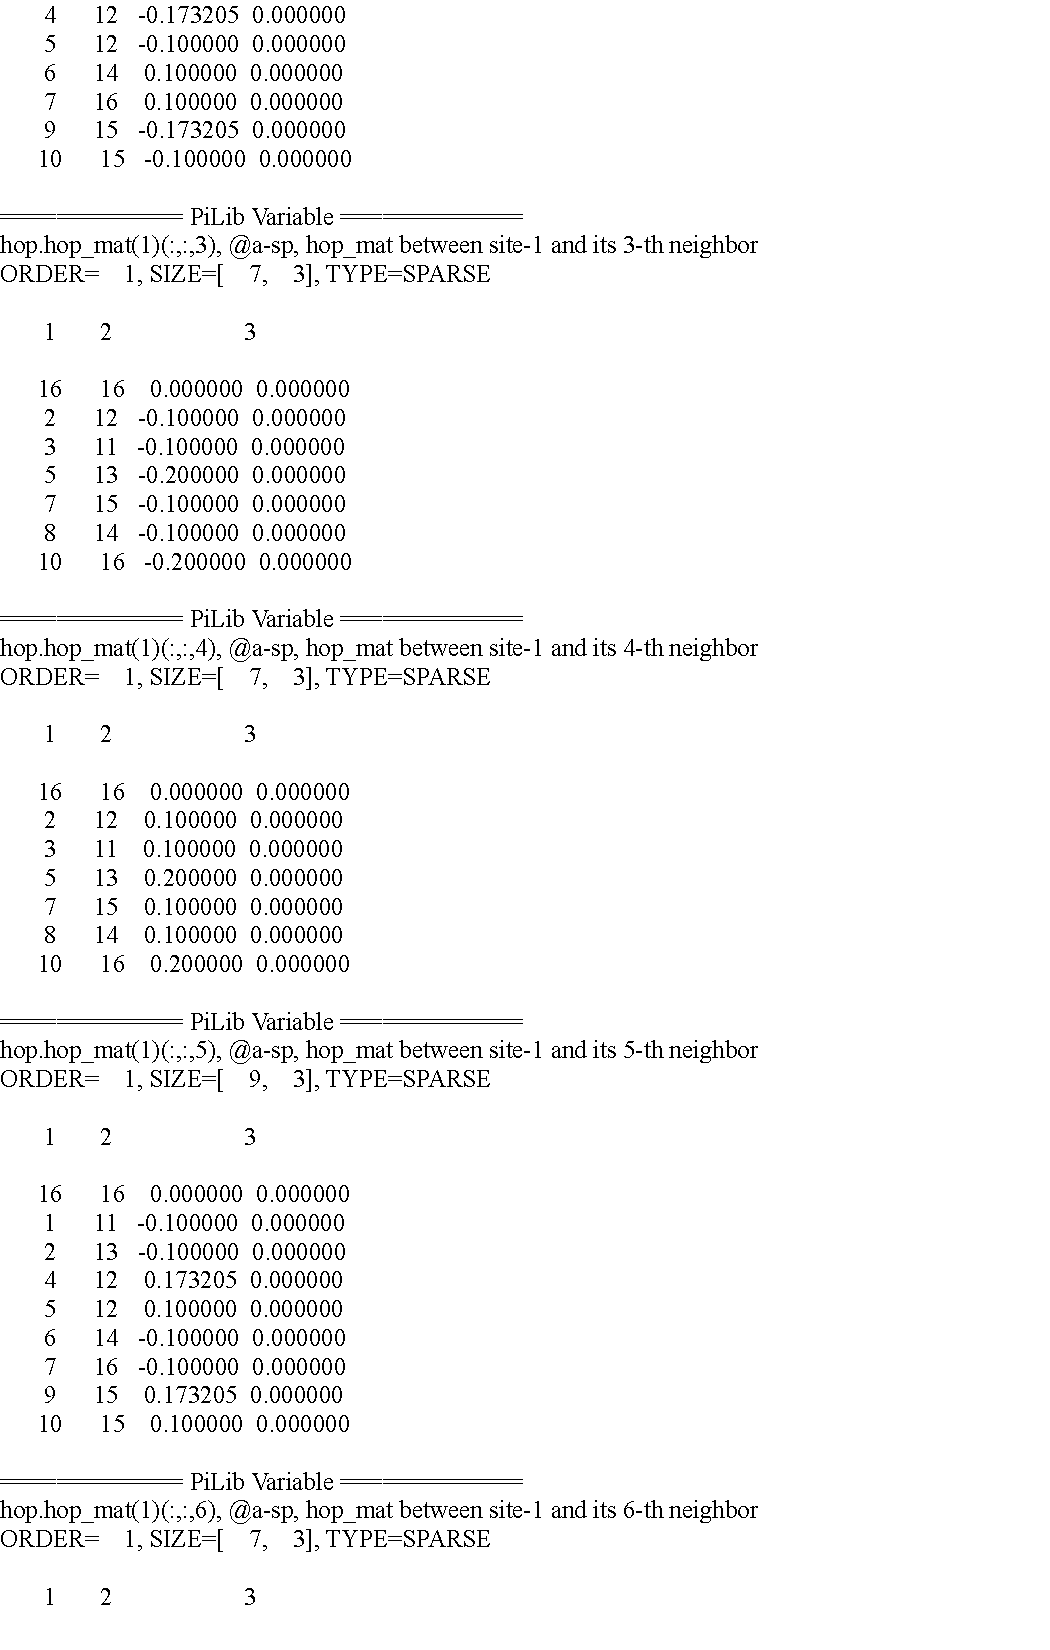
\includegraphics[width=0.9\columnwidth]{NiO_hop_p3.pdf}
\caption{page 3 of NiO\_hop.plb}
\end{figure}

\begin{figure}[tbp]
\centering
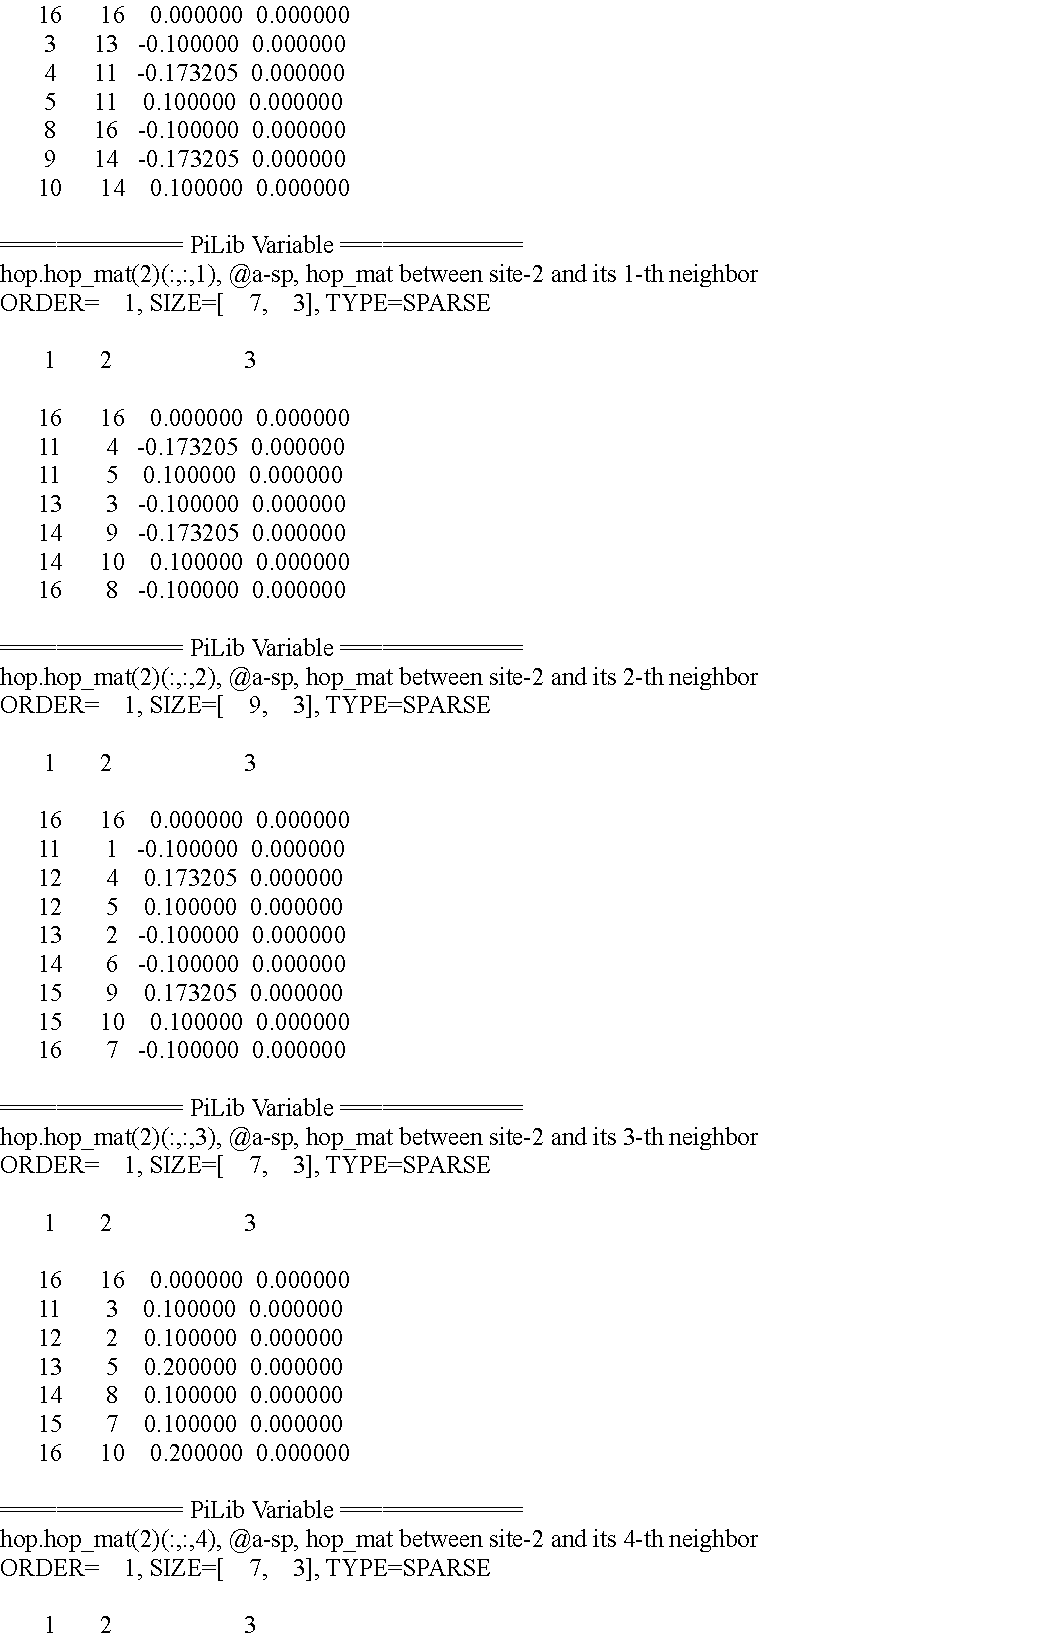
\includegraphics[width=0.9\columnwidth]{NiO_hop_p4.pdf}
\caption{page 4 of NiO\_hop.plb}
\end{figure}

\begin{figure}[tbp]
\centering
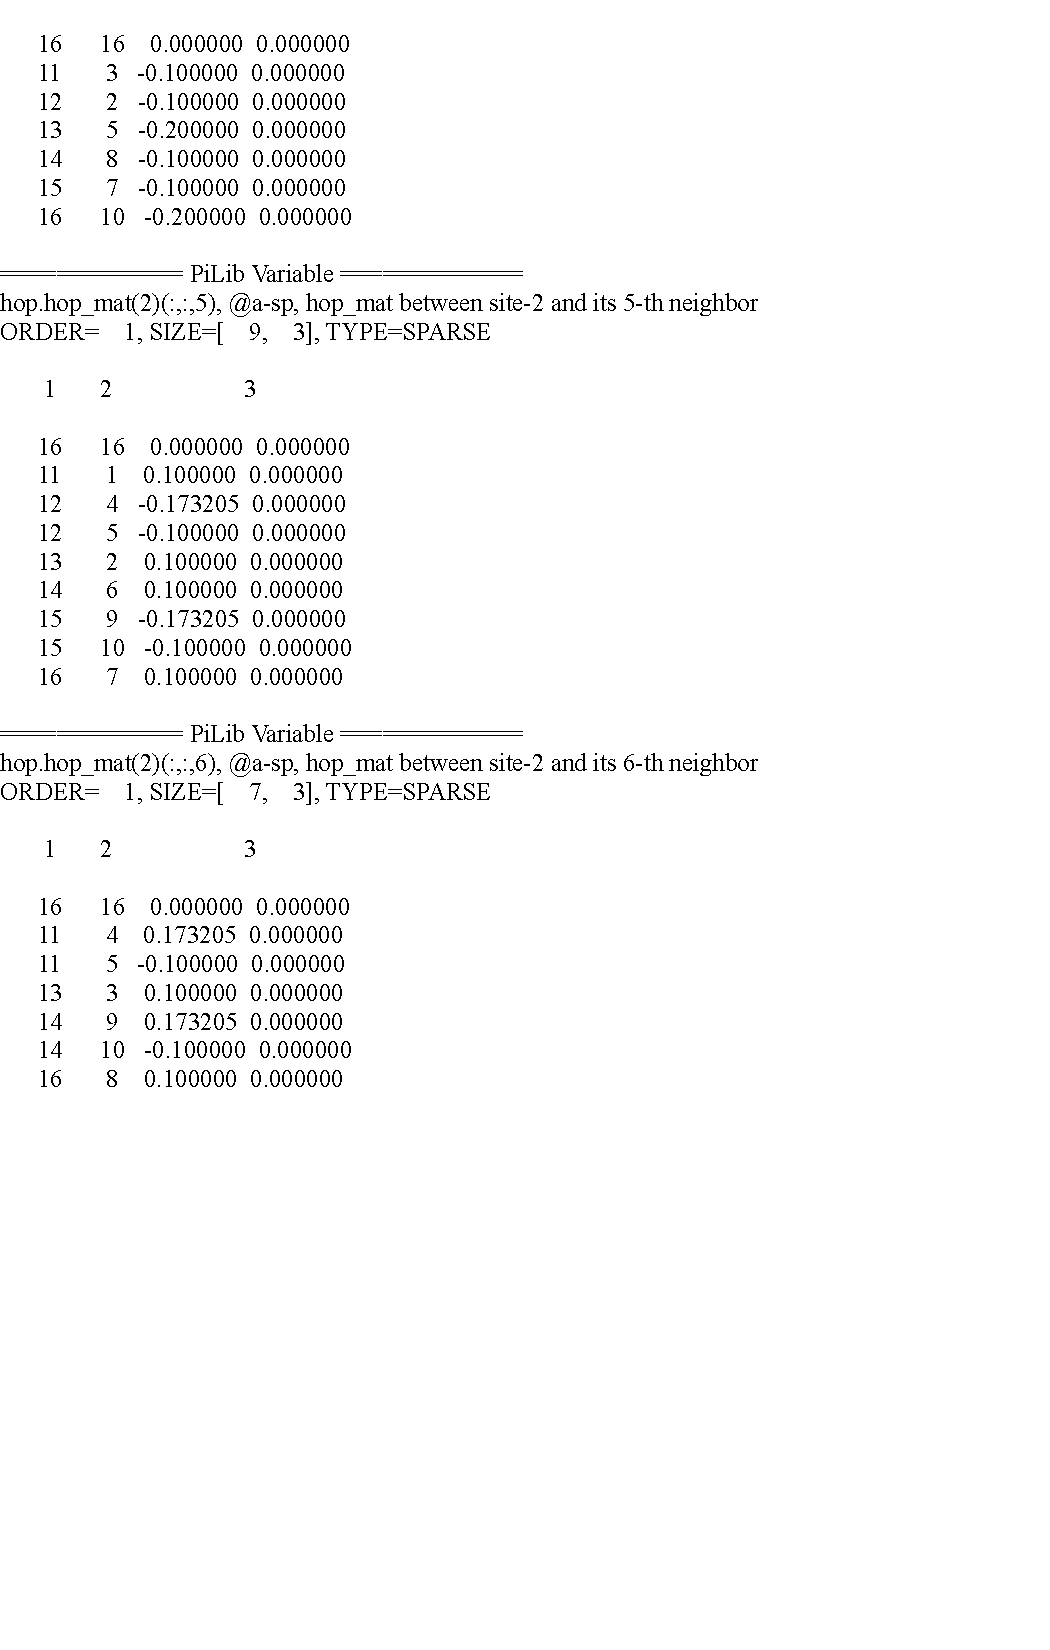
\includegraphics[width=0.9\columnwidth]{NiO_hop_p5.pdf}
\caption{page 5 of NiO\_hop.plb}
\end{figure}

\end{document}